\documentclass[a4paper,conference]{IEEEtran}
\IEEEoverridecommandlockouts

\usepackage{cite}
\usepackage{amsmath,amssymb,amsfonts}
\usepackage{textcomp}
\usepackage{url}
\usepackage{array}
\usepackage{balance}
\usepackage{tikz}
\usepackage{graphicx}
\usepackage[table]{xcolor}
\usetikzlibrary{positioning,arrows.meta,calc}

% ICAC 2026 uses double-blind review. Keep this true for the review submission.
% Set it to false only for the camera-ready paper after acceptance.
\newif\ificacblind
\icacblindtrue

\def\BibTeX{{\rm B\kern-.05em{\sc i\kern-.025em b}\kern-.08em
    T\kern-.1667em\lower.7ex\hbox{E}\kern-.125emX}}

\begin{document}

\title{SinhalaJournal-LLM: Data Centric Adaptation of a Sinhala Language Model for Journalism}
\newcommand{\systemname}{SinhalaJournal-LLM}

\ificacblind
\author{}
\else
\author{
\centering
\begin{tabular}{@{}ccc@{}}

\begin{minipage}[t]{0.305\textwidth}\centering
\textbf{Nisal Fonseka}\\
\textit{Dept. of Software Engineering}\\
\textit{Sri Lanka Institute of Information Technology}\\
Malabe, Sri Lanka\\
nisalfonseka@gmail.com
\end{minipage}
&
\begin{minipage}[t]{0.305\textwidth}\centering
\textbf{Chathushka Navod}\\
\textit{Dept. of Software Engineering}\\
\textit{Sri Lanka Institute of Information Technology}\\
Malabe, Sri Lanka\\
chathushkanavod11@gmail.com
\end{minipage}
&
\begin{minipage}[t]{0.305\textwidth}\centering
\textbf{Akash Jayasinghe}\\
\textit{Dept. of Software Engineering}\\
\textit{Sri Lanka Institute of Information Technology}\\
Malabe, Sri Lanka\\
savindu096@gmail.com
\end{minipage}
\\

\multicolumn{3}{c}{\rule{0pt}{3.2ex}} \\

\begin{minipage}[t]{0.305\textwidth}\centering
\textbf{Sandun Hettiarachchi}\\
\textit{Dept. of Software Engineering}\\
\textit{Sri Lanka Institute of Information Technology}\\
Malabe, Sri Lanka\\
lakshansandun545@gmail.com
\end{minipage}
&
\begin{minipage}[t]{0.305\textwidth}\centering
\textbf{Nuwan Kodagoda}\\
\textit{Dept. of Software Engineering}\\
\textit{Sri Lanka Institute of Information Technology}\\
Malabe, Sri Lanka\\
nuwan.k@sliit.lk
\end{minipage}
&
\begin{minipage}[t]{0.305\textwidth}\centering
\textbf{Poojani Gunathilake}\\
\textit{Dept. of Software Engineering}\\
\textit{Sri Lanka Institute of Information Technology}\\
Malabe, Sri Lanka\\
poojani.g@sliit.lk
\end{minipage}

\end{tabular}
}
\fi

\maketitle

\begin{abstract}
Sinhala has limited Natural Language Processing (NLP) support for practical
newsroom writing. This research presents \systemname, which adapts SinLlama
for grammar correction, headline generation, news summarization, and style
rewriting using separate Low-Rank Adaptation (LoRA) adapters. From 1,031,456
collected Sinhala news articles, quality filtering retained 665,887. On a
frozen 286-input grammar benchmark, SinLlama v27 achieved 56.99\% overall exact
match and corrected 63 of 143 faulty sentences, compared with 12 for
ByT5-small and none for mT5-small. Repairing grammar targets improved
development exact match from 57.8\% to 65.6\% without increasing the
36,006-row dataset. In headline generation, balancing categories before
splitting caused leakage that inflated ROUGE-1 from 0.1382 to 0.2933. Style
experiments showed persistent template repetition across generation rounds,
while only 7,555 of 22,236 synthetic candidates (34.0\%) passed the final
quality filters. The summarizer satisfied requested length bands for 44 of 45
outputs but still produced factual and numeric errors. Overall, the results
show that dataset construction, contamination control, and evaluation design
strongly affect apparent performance when adapting language models for
low-resource Sinhala generation.
\end{abstract}

\begin{IEEEkeywords}
Sinhala NLP, low-resource language, LoRA, journalism NLP, data quality
\end{IEEEkeywords}

\section{Introduction}
Large Language Models (LLMs) have improved text generation, but Sinhala still has
fewer datasets, benchmarks, and systems for specific tasks
\cite{desilva2019survey,jayakody2024performance}. SinBERT established strong
Sinhala text classification baselines \cite{dhananjaya2022bertifying}, while
SinLlama extended Llama 3 with Sinhala vocabulary and continual pretraining
\cite{grattafiori2024llama3,aravinda2025sinllama}. NSina later provided a large
Sinhala news corpus and headline generation benchmark
\cite{hettiarachchi2024nsina}.

Journalism needs several forms of constrained generation. Editors correct
language, write headlines under length limits, condense reports, and adapt the
same facts to different editorial styles. Names, numbers, dates, quotations,
and meaning must survive these operations. Sinhala studies have addressed
individual tasks such as extractive summarization \cite{jahan2023summarization}
and rule-based spelling and grammar correction \cite{goonawardena2022grammar}, but adapting one
Sinhala decoder across these connected newsroom tasks remains less explored.

\systemname{} uses SinLlama as a shared base and trains one LoRA adapter
\cite{hu2022lora} per task, with 4-bit loading to make repeated adaptation
practical on limited hardware \cite{dettmers2023qlora}. The study contributes
four task datasets derived from an original news corpus, adaptation and evaluation for each task, a frozen grammar comparison with ByT5-small and
mT5-small, a controlled grammar safety policy replay, a quantified case of
headline split leakage, and Sinhala data quality findings covering
Unicode handling, summarization decoding, and template collapse in style
rewriting. Rather than treating each component as an isolated accuracy result,
we examine how data and evaluation decisions change the apparent quality of a
low-resource generative system.

\section{Related Work}

\subsection{Sinhala Language Models and Generation Tasks}
Sinhala NLP has progressed from rule-based processing to pretrained models.
SinBERT and later Sinhala encoder models improved representation and
classification \cite{dhananjaya2022bertifying,ranasinghe2025encoder}, but are
not generative decoders. SinLlama is the closest foundation for this work.
It extends Llama 3 8B with Sinhala vocabulary and continual pretraining, then
uses LoRA for downstream classification \cite{aravinda2025sinllama}. Our work
instead studies constrained generation from the same type of decoder adapted for Sinhala.

NSina contains over 500,000 Sinhala news articles and benchmarks media
identification, category prediction, and headline generation
\cite{hettiarachchi2024nsina}. Sinhala summarization work has compared TF-IDF
and TextRank \cite{jahan2023summarization}, while multilingual sequence to sequence models such as mT5 and XL-Sum support abstractive generation
\cite{xue2021mt5,hasan2021xlsum}. Existing Sinhala spelling and grammar systems include rule-based and hybrid
approaches \cite{goonawardena2022grammar}.
These studies provide useful baselines for individual tasks but do not evaluate the four
connected editorial operations together.

\subsection{Adaptation and Evaluation of Constrained Generation}
LoRA freezes the pretrained weights and learns low-rank updates, while QLoRA
combines adapter training with a quantized base model
\cite{hu2022lora,dettmers2023qlora}. This makes separate adapters feasible
without maintaining four full 8B models. Evaluation remains task dependent.
Style transfer, for example, must balance style change, content preservation,
and fluency, for which overlap metrics alone are inadequate
\cite{ostheimer2024tst}. For this reason, each task is evaluated with measures suited to its own objective.

\section{Corpus and Task Datasets}
Project crawlers and scraping scripts collected 1,031,456 articles directly
from Sri Lankan Sinhala news sites, spanning 13 March 2008 to 4 March 2026. No
NSina data were used. Exact duplicates were removed, after which articles were
accepted only when the body contained between 300 and 10,000 characters, the title
contained between 10 and 200 characters, and at least 30\% of the characters were Sinhala Unicode. Failed rows
were discarded rather than truncated. The process removed 365,569 articles
(35.4\%), leaving 665,887. Local news and Politics were the largest categories,
with 264,434 and 151,640 articles respectively, followed by International
(68,005), Business (49,247), Sports (37,336), and Editorial (16,263). The
remaining 78,962 articles were distributed across Other, Entertainment,
Crime/Law, Health, Technology, Science, Religion, and Environment. This
distribution matters for generation experiments because the categories are
highly uneven. This can make simple category balancing
appear useful even when it creates the leakage problem demonstrated later.

\subsection{Invisible Character Handling}
Sinhala scraping exposed two visually similar characters that require different
treatment. Soft hyphen U+00AD is invisible but disrupts subword tokenization and
is removed. It appeared in 85.8\% of the rows in one style working file.
Zero width joiner U+200D participates in valid Sinhala conjuncts and is
preserved. We also observed encoding artifacts and a Devanagari danda attached
to surrounding text without whitespace in 480 of 600 inspected rows, which
broke downstream sentence splitting. The practical finding is that generic
removal of invisible or control characters can corrupt Sinhala text, so
normalization must be character aware.

\subsection{Task Datasets}
None of the tasks uses the full corpus. Each dataset was independently filtered,
transformed, and audited, as summarized in Table~\ref{tab:datasets}.

\begin{table}[!b]
\caption{Final task datasets used for adapter development}
\label{tab:datasets}
\centering
\footnotesize
\setlength{\tabcolsep}{2.6pt}
\renewcommand{\arraystretch}{1.05}
\begin{tabular}{|p{0.17\columnwidth}|p{0.25\columnwidth}|p{0.45\columnwidth}|}
\hline
\textbf{Task} & \textbf{Final data} & \textbf{Main structure} \\
\hline
Grammar & 36,006 rows & Incorrect or correct input with corrected target \\
\hline
Headline & 43,737 train, about 4,795 validation & Article, category, reference headline \\
\hline
Summary & 35,547 articles & Article with short, medium, and long summaries \\
\hline
Style & 7,555 rewrites & Article, target style, rewritten article \\
\hline
\end{tabular}
\end{table}

The summary row reports the cleaned v07 dataset. The tracked v06 model was
trained before the 22-row cleanup on 35,569 articles.

\textit{Grammar.} The final Stage 13 file contains 36,006 rows covering spelling,
verb form, agreement, word order, spacing, register, pronouns, negation,
numerals, and already correct controls. The preceding v9 and repaired v10
files contain the same 36,006 inputs in the same order. Target repair changed
4,999 rows without increasing the dataset size. This makes the later development
comparison useful for separating target quality from simple data growth.

\textit{Headline.} The final v19 training set contains 43,737 rows with short
(3 to 5 words), medium (6 to 7 words), and long (8 to 10 words) target bands. Earlier category
balancing physically duplicated minority examples. Section VI-B shows that
performing this before the split caused leakage. Later targets were cleaned of
media and scraper artifacts.

\textit{Summarization.} The v06 silver corpus contains 35,569 articles, each
paired with short, medium, and long summaries targeted at approximately 10\%,
20\%, and 35\% of source length. A follow-up audit removed 22 records with
word joining, number and unit, or unrelated content faults, producing a 35,547-row
v07 cleaned file. A v07 adapter was trained and evaluated on this cleaned file
using the same 45-output protocol as the tracked v06 evaluation reported
below. That protocol resamples articles from the training corpus itself
rather than a persisted, article-level held-out split, so neither the v06 nor
the v07 result under it is a reliable basis for choosing between the two
versions; Section VI-D and the Limitations discuss this and a leakage-controlled
re-evaluation in progress.

\textit{Style rewriting.} The cleaned dataset contains 7,555 rewrites across
formal news, editorial, sports, youth, and feature styles. A generation audit
accepted 7,555 of 22,236 candidates (34.0\%) after structural, factual, script,
length, and copy checks. Repeated sequences, missing closings, numeric changes,
and incorrect gender honorifics were among the detected faults. Outputs
were also required to keep a length ratio between 0.7 and 1.4 and remain below 0.80 source
similarity, directly addressing the copying failure discussed in Section VI-D.

\section{Model Adaptation and Fine-Tuning}

\subsection{Base Model}
SinLlama is the common base. We begin from the model already adapted for Sinhala rather than
repeating its tokenizer extension or continual pretraining
\cite{aravinda2025sinllama}. The merged checkpoint is loaded in 4-bit NF4 with
BF16 compute, and each task uses a separate LoRA adapter. Fig.~\ref{fig:modeladaptation}
summarizes the relationship. The summarizer node in Fig.~\ref{fig:modeladaptation}
names v07 because the serving layer automatically deploys whichever
version-numbered adapter folder is highest, independent of any quality
comparison; this is a deployment fact, not evidence that v07 was selected on
merit, and is separate from which version the results in Section VI-D treat
as the tracked baseline.

\begin{figure}[!t]
\centering
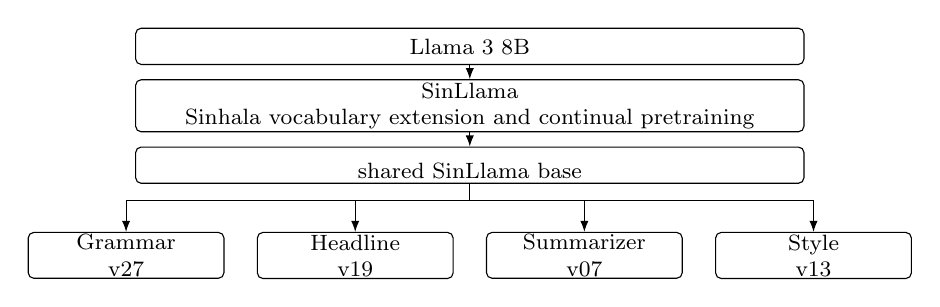
\begin{tikzpicture}[
    base/.style={draw, rounded corners=2pt, align=center,
        minimum width=0.70\columnwidth, minimum height=4.6mm,
        inner sep=1.1pt, font=\footnotesize},
    adapter/.style={draw, rounded corners=2pt, align=center,
        minimum width=0.205\columnwidth, minimum height=4.8mm,
        inner sep=0.8pt, font=\footnotesize},
    flow/.style={-{Latex[length=1.4mm]}, line width=0.4pt},
    branchline/.style={line width=0.4pt}
]
\node[base] (llama) {Llama 3 8B};
\node[base, below=1.8mm of llama] (sinllama)
    {SinLlama\\Sinhala vocabulary extension and continual pretraining};
\node[base, below=1.8mm of sinllama] (shared)
    {\systemname{}\\shared SinLlama base};

\node[adapter, below=6.1mm of shared, xshift=-0.36\columnwidth] (grammar)
    {Grammar\\v27};
\node[adapter, below=6.1mm of shared, xshift=-0.12\columnwidth] (headline)
    {Headline\\v19};
\node[adapter, below=6.1mm of shared, xshift=0.12\columnwidth] (summary)
    {Summarizer\\v07};
\node[adapter, below=6.1mm of shared, xshift=0.36\columnwidth] (style)
    {Style\\v13};

\draw[flow] (llama) -- (sinllama);
\draw[flow] (sinllama) -- (shared);
\coordinate (branch) at ($(shared.south)+(0,-2.1mm)$);
\coordinate (gbranch) at (grammar.north |- branch);
\coordinate (hbranch) at (headline.north |- branch);
\coordinate (sbranch) at (summary.north |- branch);
\coordinate (tbranch) at (style.north |- branch);
\draw[branchline] (shared.south) -- (branch);
\draw[branchline] (gbranch) -- (tbranch);
\draw[flow] (gbranch) -- (grammar.north);
\draw[flow] (hbranch) -- (headline.north);
\draw[flow] (sbranch) -- (summary.north);
\draw[flow] (tbranch) -- (style.north);
\end{tikzpicture}
\caption{Model adaptation architecture of \systemname{}.}
\label{fig:modeladaptation}
\end{figure}

\subsection{Prompt Design}
Prompts encode the constraints later evaluated. Grammar instructs the model to
fix only errors and return correct text unchanged. Headline prompts include
category and requested word band. Summarization uses instructions for each requested length that restrict content to the source. Style uses a target style
instruction with factual preservation rules for entities, numbers, dates,
quotations, honorifics, and unsupported substitutions. We therefore treat the
prompt as part of the task definition rather than only an interface wrapper.

\subsection{LoRA Configuration}
All adapters target the same seven attention and MLP projections and use seed
42 with validation loss checkpoint selection. Table~\ref{tab:config} records
the selected configurations used in the reported development runs. Grammar
v27 deliberately reduces rank from 32 to 4 as a capacity experiment. The
result did not improve transfer to untaught correction pairs. For summarization, v06 is shown
as the primary tracked configuration; v07 uses an identical configuration on
the cleaned data and has also been trained and evaluated, but its evaluation
shares the same small-sample, non-blind protocol as v06's and is not yet used
to select between the two versions (Section VI-D).

\begin{table*}[!t]
\caption{Selected LoRA fine-tuning configurations used in the reported task experiments. All use seed 42, a 4-bit NF4 SinLlama base with BF16 compute, and the same seven target projections.}
\label{tab:config}
\centering
\footnotesize
\setlength{\tabcolsep}{4pt}
\renewcommand{\arraystretch}{1.08}
\begin{tabular}{|l|l|r|c|r|c|c|c|r|}
\hline
\textbf{Task} & \textbf{Adapter} & \textbf{Train rows} & \textbf{$r$\,/\,$\alpha$\,/\,dropout} &
\textbf{Max seq.} & \textbf{Eff. batch} & \textbf{LR} & \textbf{Epochs} & \textbf{Trainable params} \\
\hline
Grammar       & v27 & 36,006 & 4\,/\,4\,/\,0.05    & 512  & 8  & 5e-5 & 3.00 (pinned)  & 10,485,760 \\
\hline
Headline      & v19 & 43,737 & 64\,/\,128\,/\,0.08 & 768  & 8  & 5e-5 & 8 (early stop) & 167,772,160 \\
\hline
Summarization & v06 & 35,569 & 32\,/\,64\,/\,0.05  & 2048 & 16 & 2e-4 & 3              & 83,886,080 \\
\hline
Style         & v13 & 7,555  & 24\,/\,48\,/\,0.05  & 4096 & 16 & 1e-4 & 3              & 62,914,560 \\
\hline
\end{tabular}
\end{table*}

\subsection{Inference Configuration}
Grammar and style use deterministic decoding. Headline generation samples at
temperature 0.3 and top-$p$ 0.9 with a retry when the first output is too short. Summarization uses
deterministic decoding and separate token limits for each requested length. An earlier
\texttt{no\_repeat\_ngram\_size=3} setting was removed after it corrupted
opening Sinhala grapheme sequences, showing that decoding constraints commonly
used for other languages are not automatically safe for Sinhala.

\textit{Reproducibility and data use.} Grammar v27 was trained on one NVIDIA
A40 for 6.36 hours with 44.352 GB peak GPU memory. Runtime logs for the other
adapters were not retained. The corpus came from publicly accessible news pages
for academic research, and full article text is not redistributed in this
manuscript. Repository links are omitted for double-blind review. The exact
teacher provider for the tracked v06 summaries was not persisted, which remains
a reproducibility limitation.

\section{Evaluation Protocol}
The four tasks use different definitions of correctness. The frozen grammar benchmark (Stage 6) is a
manually reviewed set of 286 unseen inputs. It contains
143 cases that require a change and 143 correct controls. No input overlaps the
final training data or Stage 5 after normalization, and 87 changed cases contain
exact correction pairs absent from training. We report overall and
exact match on cases requiring changes, clean preservation, edit precision and recall,
$F_{0.5}$, and unseen pair recall. The same inputs are given to SinLlama v27 and
v25, ByT5-small \cite{xue2022byt5}, and mT5-small \cite{xue2021mt5}.

Two additional grammar analyses are explicitly developmental rather than new
blind tests. First, the grammar development benchmark (Stages 2 to 5) provides 154 examples
for comparing taught and untaught correction pairs and the v24 to v27 versions. Second, the
same 154 saved v27 predictions are replayed through the neural output alone, rules alone, the
legacy hybrid, and the recalibrated hybrid. Because the neural
candidate is fixed, this replay isolates policy effects, but the benchmark had
already influenced development and is not an independent estimate of newsroom
performance.

Headline evaluation uses the repaired 4,795 example split to diagnose category
leakage, then evaluates v18 to v20 on 300 articles at all three requested length
bands, giving 900 outputs per version. We report overlap, requested length
accuracy, artifact rate, and counts for each category. A separate 100 article
publisher set provides a limited transfer check.

Summarization uses ROUGE calculated on Sinhala graphemes as an internal
diagnostic \cite{lin2004rouge}. The tracked v06 evaluation contains 15 articles
generated at three lengths, for 45 outputs. Because this is a small evaluation
without an independent article-level blind split, the main reported result is
length control. We report target and observed compression, compliance with the
requested length band, and whether generation ends cleanly. Teacher data audits
and stored predictions are inspected separately for factual errors and errors
involving numbers and units. The later v07
cleaning recipe is described as data preparation only because no saved v07
model result is available.

Style rewriting combines overlap, cosine similarity, source divergence, length
preservation, and target audits because high overlap can reward unchanged text.
Discarded targets were compared across two generation rounds for repeated style
phrases and near-verbatim copying above 0.90 character similarity. A v13
development diagnostic sampled 15 items per style (75 outputs). Its composite
score is retained only as an internal aid because the sample is not a frozen
independent benchmark.

\section{Results and Discussion}
\subsection{Grammar Correction}
Table~\ref{tab:grammar} shows the Stage 6 comparison. v25 and v27 both correct
63 of 143 faulty sentences. v25 preserves one additional clean control. The clustered 95\% interval is 50.35\% to 64.69\% for v25 and 50.00\%
to 63.99\% for v27. The intervals overlap substantially, so the difference of
one example is not evidence that either version is generally superior. v27 is
retained as the final grammar adapter.

\begin{table}[!t]
\caption{Grammar Stage 6 comparison on 286 unseen inputs}
\label{tab:grammar}
\centering
\footnotesize
\setlength{\tabcolsep}{1.9pt}
\renewcommand{\arraystretch}{1.04}
\begin{tabular}{|l|r|r|r|r|}
\hline
\textbf{System} & \textbf{Overall} & \textbf{Change} & \textbf{$F_{0.5}$} & \textbf{Unseen} \\
\hline
SinLlama final (v27) & 56.99\% & 44.06\% & 45.36\% & 40.23\% \\
\hline
SinLlama prior (v25) & 57.34\% & 44.06\% & 46.21\% & 41.38\% \\
\hline
ByT5-small v01 & 50.00\% & 8.39\% & 20.34\% & 13.79\% \\
\hline
mT5-small v01 & 50.00\% & 0.00\% & 0.00\% & 0.00\% \\
\hline
\end{tabular}
\end{table}

ByT5-small repairs only 12 faulty inputs and damages 12 clean controls, leaving
its overall score equal to the unchanged input baseline. The mT5-small result after safety filtering is also the unchanged baseline. SinLlama is therefore much
stronger at making required corrections, but v27 still reaches only 40.23\%
unseen pair recall and preserves 69.93\% of clean controls. The remaining
problem is not only correction ability but transfer and restraint.

The development history explains this more clearly. Table~\ref{tab:gdev}
uses the same current gold for v24 to v27. All four runs use 36,006 rows. v24 and
v26 also keep rank 32 and approximately the same three epoch budget. The main
data change is the repair of the target outputs. Under these nearly matched
conditions, aggregate exact match rises from 57.8\% in v24 to 65.6\% in v26.

\begin{table}[!t]
\caption{Grammar development diagnostic on Stages 2 to 5}
\label{tab:gdev}
\centering
\footnotesize
\setlength{\tabcolsep}{2.2pt}
\renewcommand{\arraystretch}{1.03}
\begin{tabular}{|l|c|c|r|r|r|}
\hline
\textbf{Ver.} & \textbf{Targets} & \textbf{Rank} & \textbf{Exact} & \textbf{Taught} & \textbf{Untaught} \\
\hline
v24 & older & 32 & 57.8\% & 88\% & 42\% \\
\hline
v25 & repaired & 32 & 66.2\% & 91\% & 50\% \\
\hline
v26 & repaired & 32 & 65.6\% & 91\% & 47\% \\
\hline
v27 & repaired & 4 & 66.9\% & 91\% & 48\% \\
\hline
\end{tabular}
\end{table}

The table also shows that the remaining limitation is transfer rather than raw
capacity. v27 uses rank 4, about one eighth of the trainable adapter parameters
of the rank 32 runs, yet its aggregate exact match remains comparable. However,
its untaught pair score stays at 48\% while taught pairs reach 91\%. The rank
reduction therefore improves parameter efficiency but does not force the model
to learn a general correction rule. This is why we treat target quality and
coverage of correction patterns as stronger explanations than adapter size.

Earlier stages show why these harder diagnostics were necessary. v19 reached
93\% on Stage 2 and 90\% on Stage 3, but fell to 58.3\% when Stage 4 moved to
real published articles. High scores on short, familiar tests therefore did not
translate directly to harder news text. Training behavior gave a similar
pattern. The v25 evaluation loss reached its minimum at the end of epoch 3 and rose
through epoch 4, which motivated the pinned three epoch budget used later. The
project also moved from loss over the full sequence to loss only on the completion after v13
and v14 returned identical Stage 2 results despite additional data. We treat
these as development diagnostics rather than independent ablations, because
several training variables changed across the early versions.

The grammar pipeline also includes a rule validator, and Table~\ref{tab:hybrid}
reports a controlled replay using the same 154 saved v27 predictions. Rules
alone preserve clean text but correct none of the 116 faulty examples. The
legacy policy treats too many warnings as vetoes and suppresses 23
candidate edits, lowering neural edit recall from 71.14\% to 56.22\%
and exact match from 66.88\% to 57.14\%. Recalibration restores the neural exact
match and recall, raises edit precision from 88.27\% to 88.82\%, and reduces the
unsupported entity error from 0.65\% to 0\%. Number error remains 0\%.
The result supports rules as a selective safety layer, not as a replacement
corrector or a blanket veto. Because policy design used this development set,
it is an ablation of validator behavior rather than an independent benchmark.

\begin{table}[!b]
\caption{Grammar validator replay on 154 development examples}
\label{tab:hybrid}
\centering
\footnotesize
\setlength{\tabcolsep}{2.3pt}
\renewcommand{\arraystretch}{1.03}
\begin{tabular}{|l|r|r|r|}
\hline
\textbf{System} & \textbf{Exact} & \textbf{Edit recall} & \textbf{Unsup. entity} \\
\hline
Neural v27 & 66.88\% & 71.14\% & 0.65\% \\
\hline
Rules only & 24.68\% & 0.00\% & 0.00\% \\
\hline
Legacy hybrid & 57.14\% & 56.22\% & 0.00\% \\
\hline
Recalibrated hybrid & 66.88\% & 71.14\% & 0.00\% \\
\hline
\end{tabular}
\end{table}

\subsection{Category Balancing Introduced Leakage}
\label{sec:leak}
An early headline dataset balanced minority categories by physical duplication
before the training and validation split. Copies of the same article therefore entered
both partitions. The leaked evaluation reported ROUGE-1 of 0.2933 and 485 exact
matches among 6,732 outputs, while the repaired split reported 0.1382 and no
exact matches among 4,795 outputs.

\begin{table}[!b]
\caption{ROUGE-1 by category before and after repairing the split. Duplication factor is the upsampled validation count divided by the genuine count. }
\label{tab:leak}
\centering
\footnotesize
\setlength{\tabcolsep}{3pt}
\renewcommand{\arraystretch}{1.04}
\begin{tabular}{|l|r|r|r|r|}
\hline
\textbf{Category} & \textbf{Genuine $n$} & \textbf{Dup.} & \textbf{Leaked} & \textbf{Repaired} \\
\hline
\rowcolor{gray!10}
\textbf{Technology} & \textbf{10} & \textbf{40.0$\times$} & \textbf{0.7275} & \textbf{0.1320} \\
\hline
Human Rights  & 14  & 28.6$\times$ & 0.6295 & 0.0562 \\
\hline
Health        & 48  & 8.3$\times$  & 0.6044 & 0.1467 \\
\hline
Science       & 75  & 5.3$\times$  & 0.4843 & 0.1014 \\
\hline
Editorial     & 86  & 4.7$\times$  & 0.6339 & 0.0338 \\
\hline
Law and Order & 230 & 1.7$\times$  & 0.2422 & 0.1157 \\
\hline
Sports        & 722 & 1.0$\times$  & 0.1713 & 0.1646 \\
\hline
Politics      & 722 & 1.0$\times$  & 0.1502 & 0.1292 \\
\hline
\end{tabular}
\end{table}

Table~\ref{tab:leak} makes the mechanism visible. Technology had only ten
genuine validation articles, was duplicated 40 times and reached 0.7275.
Sports and Politics required no duplication and changed little after repair.
The practical lesson is to split before balancing and to report genuine
category counts together with scores. The combination of a very small genuine count
and an unusually high score exposed the fault.
The overall ROUGE value alone did not show the problem. Style training consequently uses weighted
sampling rather than duplicated rows, preserving the minority style sampling
probability without creating identical articles on both sides of its split.

\subsection{Headline Generation}
Table~\ref{tab:headline} compares the adapters for the three requested lengths after leakage
repair. v18 has the highest length accuracy, but 11.2\% of its outputs contain
media artifacts. Cleaning target headlines in v19 reduces this to 1.1\% while
length accuracy falls only from 80.9\% to 79.7\%. In v18 the artifact rate
rises from 0.3\% for short headlines to 22.3\% for long ones, consistent with
scraped suffixes fitting more easily inside wider word budgets.

\begin{table}[!t]
\caption{Headline results across 900 outputs per version, shown as accuracy within the requested band / artifact rate}
\label{tab:headline}
\centering
\footnotesize
\setlength{\tabcolsep}{2.2pt}
\renewcommand{\arraystretch}{1.04}
\begin{tabular}{|l|c|c|c|c|c|}
\hline
\textbf{Ver.} & \textbf{Short} & \textbf{Medium} & \textbf{Long} & \textbf{Overall} & \textbf{R-1 / R-L} \\
\hline
v18 & 88.7 / 0.3 & 76.0 / 11.0 & 78.0 / 22.3 & 80.9 / 11.2 & 0.124 / 0.121 \\
\hline
\textbf{v19} & 89.7 / \textbf{0.0} & 74.3 / 0.3 & 75.0 / 3.0 & 79.7 / \textbf{1.1} & 0.134 / 0.130 \\
\hline
v20 & 84.7 / 0.3 & 75.3 / 1.0 & 79.7 / 2.3 & 79.9 / 1.2 & 0.139 / 0.136 \\
\hline
\end{tabular}
\end{table}

v20 additionally cleans article inputs, but its validation input is already
clean, so the test cannot observe the copying behavior it was designed to
remove. We therefore retain v19 rather than reading v20's slightly higher
ROUGE as evidence for the input cleaning hypothesis. On 100 articles from a
publisher that was not used for training, v17 reaches ROUGE-1 0.1567 but a length ratio of 0.81,
showing reasonable lexical transfer while generating shorter headlines than the references from a different
house style.

\subsection{Style Rewriting and Synthetic Target Quality}
Two discarded style-target generation rounds exposed a systematic teacher-side
failure. Repeated style-specific phrases remained almost unchanged despite a
more than fivefold increase in generation volume: editorial changed from
55.6\% to 56.1\%, youth from 61.1\% to 61.9\%, and feature from 49.7\% to
49.2\%. Formal news and sports instead showed 15\% to 17\% near-verbatim
targets, while a separate audit found full-source containment in 94.3\% of an
early target file. The trained adapter reproduced these defects, indicating
that increasing synthetic data volume did not correct a defective target
distribution.

The targets were regenerated and filtered for copying, repetition, factual
consistency, structure, script, and length. Only 7,555 of 22,236 candidates
(34.0\%) were retained. In a later 75-output v13 development diagnostic, the
mean source-divergence score was 29.1\% for formal news and sports combined but
52.7\% for editorial, youth, and feature combined; individual cases reached
92.6\% divergence even though verbatim copying fell to 0\%. This suggests that
cleaning removed the obvious copy failure while stronger transformations
remained more vulnerable to semantic drift. Because the diagnostic was not a
frozen independent benchmark, we do not report its composite score as final
style accuracy.

\subsection{News Summarization}
The tracked v06 evaluation contains 15 articles at each of three requested
lengths. Table~\ref{tab:summary} shows that length conditioning is effective.
Mean compression is 0.118, 0.231, and 0.363 for targets of about 10\%, 20\%,
and 35\%. A total of 44 of 45 outputs fall inside the requested band, and all
45 outputs end cleanly rather than being cut off in the middle of a sentence.
Grapheme-based ROUGE was also computed for internal analysis, but we do not
present it as an independent estimate of summarization quality because the
evaluation is small and not article-level blind.

\begin{table}[!b]
\caption{Tracked v06 length-control results, 15 articles per length}
\label{tab:summary}
\centering
\footnotesize
\setlength{\tabcolsep}{3.2pt}
\renewcommand{\arraystretch}{1.03}
\begin{tabular}{|l|r|r|r|r|}
\hline
\textbf{Length} & \textbf{Target} & \textbf{Observed} & \textbf{In band} & \textbf{Clean end} \\
\hline
Short  & 0.10 & 0.1177 & 93.33\% & 100\% \\
\hline
Medium & 0.20 & 0.2313 & 100\% & 100\% \\
\hline
Long   & 0.35 & 0.3629 & 100\% & 100\% \\
\hline
\end{tabular}
\end{table}

The result is useful because it separates controllability from factuality. The
model follows the requested compression ratios closely and terminates cleanly,
but a stored long prediction changes a reference to Portugal and Uruguay into Pakistan.
The teacher data audit also found 21 genuine word joining or number and unit
errors, together with one false positive. Some of these errors changed the
reported scale by 100 to 1000 times. These faults matter in news because a fluent summary can still alter the
actor, country, or magnitude of the event.

The v07 data cleaning pass removes 22 suspect rows from the 35,569-row silver
corpus, producing 35,547 rows. A v07 adapter was trained and evaluated on
this cleaned corpus using the same 45-output protocol as the v06 result
above; on that protocol v07 scores a lower ROUGE-L in all three bands (e.g.
0.549 vs.\ 0.488 for long summaries) and a mixed in-band rate relative to
v06. However, a contamination audit of both adapters' original training
splits against a newly constructed, article-level held-out test set found
that roughly 81\% of that held-out set was already present in each
adapter's original training data — a direct consequence of splitting at the
sample level (Section~\ref{sec:leak} describes an analogous leakage
mechanism for headline data). Neither the v06 nor the v07 number above should
therefore be read as a quality comparison; a leakage-controlled
re-evaluation using the frozen split is planned but not yet complete. We
report the cleaning itself as a dataset improvement and do not yet claim
that it raises ROUGE or factual accuracy. An earlier standard no-repeat n-gram
constraint also corrupted opening Sinhala grapheme sequences and was removed.
This is an important Sinhala specific observation. A decoding constraint intended to
reduce repetition can also damage Sinhala grapheme sequences.

The evaluation remains small and limited to one source family. The three length
variants are created before the 85/15 split, so variants of one article can
cross partitions. The evaluator also samples from the silver corpus rather than
a persisted blind set. The v06 results therefore demonstrate length control,
not generalization to an independent publisher.

A similar issue appeared across all four components. Grammar improved after
target repair without increasing dataset size. Headline duplication inflated
ROUGE. Style filtering removed the obvious copy failure, but the development
diagnostic still showed greater semantic drift in more transformative styles.
The summarizer controlled length while factual defects remained. These results
show that dataset construction and evaluation must be checked before a higher
model score is treated as an improvement.

\section{System Integration}
The four tasks are available through web, browser, and Google Docs clients.
Requests go to a FastAPI backend that selects the required preprocessing and
LoRA adapter on the shared SinLlama server. Grammar can revert unsafe edits,
while headline output cleaning removes media tags. A combined system accuracy
is not reported because the four tasks have different objectives.

\section{Limitations and Future Work}
Evaluation strength differs across the four components. Grammar Stage 6 is the
strongest comparison, but it uses local news material and unseen pair recall is
still about 40\%. The 154 example grammar analyses are development experiments,
not additional blind tests.

Headline transfer was tested on one external publisher, and v20 still needs
evaluation on the dirty inputs it was designed to clean. Summarization uses only
15 articles and lacks an article-level blind split.
% TODO(SUMMARIZATION_NEXT_STEPS.md): an article-level frozen train/val/test
% split now exists, and a contamination audit found ~81% overlap between it
% and both existing adapters' original training data. Replace this
% limitation once the frozen-split retrain and re-evaluation (in progress)
% produce a tracked result.
Style has only a 75-output
development diagnostic sampled from the labeled dataset rather than a frozen
independent benchmark, and its training and serving prompts are different.

Future work will use larger human reviewed sets from independent publishers,
add contextual grammar and factual checks, and isolate articles before the
summarization split. A separate user evaluation with journalists, media
students, and Sinhala language experts will assess editorial usefulness.

\balance
\section{Conclusion}
\systemname{} adapts one Sinhala decoder to four newsroom tasks using separate LoRA
adapters. On Stage 6, SinLlama corrects 63 of 143 faulty grammar inputs, compared
with 12 for ByT5-small and none for mT5-small. Transfer to unseen correction
pairs is still limited. Repairing the grammar targets also improved development
exact match from 57.8\% to 65.6\% under nearly the same training conditions.
The revised rule validator removed the observed unsupported entity error without
reducing neural recall. Headline balancing before the split more than doubled
the apparent ROUGE-1 score because duplicated articles entered validation. Style experiments showed that increasing synthetic generation volume did not
remove systematic template collapse; only 34.0\% of generated candidates
passed the final quality filters, while stronger transformations remained more
vulnerable to semantic drift. The summarizer controlled length well but still
showed factual and number related errors. The
main result across the four tasks is that data quality and evaluation design
strongly affect measured performance. Increasing adapter capacity alone did
not solve these problems.

\ificacblind
\else
\section*{Acknowledgment}
The authors thank the Faculty of Computing, Sri Lanka Institute of Information
Technology, for the supervision, guidance, and computing resources provided
throughout this research project.
\fi

\begin{thebibliography}{00}
\bibitem{desilva2019survey} N. de Silva, ``Survey on publicly available Sinhala natural language processing tools and research,'' arXiv:1906.02358, 2019.
\bibitem{jayakody2024performance} R. Jayakody and G. Dias, ``Performance of recent large language models for a low-resourced language,'' in \textit{Proc. Int. Conf. Asian Language Processing (IALP)}, 2024, pp. 162--167, doi: 10.1109/IALP63756.2024.10661169.
\bibitem{dhananjaya2022bertifying} V. Dhananjaya, P. Demotte, S. Ranathunga, and S. Jayasena, ``BERTifying Sinhala - a comprehensive analysis of pre-trained language models for Sinhala text classification,'' in \textit{Proc. LREC}, 2022, pp. 7377--7385.
\bibitem{grattafiori2024llama3} A. Grattafiori \textit{et al.}, ``The Llama 3 herd of models,'' arXiv:2407.21783, 2024.
\bibitem{aravinda2025sinllama} H. W. K. Aravinda \textit{et al.}, ``SinLlama - a large language model for Sinhala,'' in \textit{Proc. Moratuwa Eng. Res. Conf. (MERCon)}, 2025, pp. 617--622, doi: 10.1109/MERCon67903.2025.11217094.
\bibitem{hettiarachchi2024nsina} H. Hettiarachchi, D. Premasiri, L. Uyangodage, and T. Ranasinghe, ``NSina: A news corpus for Sinhala,'' in \textit{Proc. LREC-COLING}, 2024.
\bibitem{jahan2023summarization} M. A. C. Akmal Jahan and K. K. C. Wijesekara, ``Automated text summarization of Sinhala online articles,'' \textit{J. Science-FAS-SEUSL}, vol. 4, no. 1, pp. 1--15, 2023.
\bibitem{goonawardena2022grammar} M. Goonawardena, A. Kulatunga, R. Wickramasinghe, T. Weerasekara, H. De Silva, and S. Thelijjagoda, ``Automated spelling checker and grammatical error detection and correction model for Sinhala language,'' in \textit{Proc. Int. Res. Conf. Smart Computing and Systems Engineering (SCSE)}, 2022, pp. 184--189, doi: 10.1109/SCSE56529.2022.9905126.
\bibitem{hu2022lora} E. J. Hu \textit{et al.}, ``LoRA: Low-rank adaptation of large language models,'' in \textit{Proc. ICLR}, 2022.
\bibitem{dettmers2023qlora} T. Dettmers, A. Pagnoni, A. Holtzman, and L. Zettlemoyer, ``QLoRA: Efficient finetuning of quantized LLMs,'' in \textit{Advances in Neural Information Processing Systems}, 2023.
\bibitem{ranasinghe2025encoder} T. Ranasinghe \textit{et al.}, ``Sinhala encoder-only language models and evaluation,'' in \textit{Proc. 63rd ACL}, 2025, pp. 8623--8636.
\bibitem{xue2021mt5} L. Xue \textit{et al.}, ``mT5: A massively multilingual pre-trained text-to-text transformer,'' in \textit{Proc. NAACL-HLT}, 2021, pp. 483--498.
\bibitem{hasan2021xlsum} T. Hasan \textit{et al.}, ``XL-Sum: Large-scale multilingual abstractive summarization for 44 languages,'' in \textit{Findings of ACL-IJCNLP}, 2021, pp. 4693--4703.
\bibitem{ostheimer2024tst} P. S. Ostheimer, M. K. Nagda, M. Kloft, and S. Fellenz, ``Text style transfer evaluation using large language models,'' in \textit{Proc. LREC-COLING}, 2024, pp. 15802--15822.
\bibitem{xue2022byt5} L. Xue \textit{et al.}, ``ByT5: Towards a token-free future with pre-trained byte-to-byte models,'' \textit{Trans. Assoc. Comput. Linguistics}, vol. 10, pp. 291--306, 2022.
\bibitem{lin2004rouge} C.-Y. Lin, ``ROUGE: A package for automatic evaluation of summaries,'' in \textit{Text Summarization Branches Out}, 2004, pp. 74--81.
\end{thebibliography}

\end{document}
